\documentclass[a4j,12pt]{jsreport}
% 数式
\usepackage{amsmath,amsfonts}
\usepackage{bm}

% 画像
\usepackage[dvipdfmx]{graphicx}

% biblatex
\usepackage[style=numeric, sorting=none, maxbibnames=1000]{biblatex}
\addbibresource{graduation_thesis.bib}

%itembox
\usepackage{ascmac}
%breakitemboxのためのpackage
\usepackage{itembkbx}
% \usepackage{tcolorbox} 画像が見えなくなってしまう原因
% \usepackage{framed} 枠

%フォント
\usepackage[ipaex]{pxchfon}

\usepackage[top=35truemm,bottom=30truemm,left=30truemm,right=30truemm]{geometry}
\usepackage{float}
\usepackage{multicol}
\usepackage{multirow}
\usepackage{paralist}
\usepackage{caption}
\usepackage{setspace}
\usepackage{algorithm}
\usepackage{algpseudocode}
\usepackage[dvipdfmx,hidelinks]{hyperref}
\usepackage{pxjahyper}
\usepackage{fancyhdr}
\usepackage{ltablex}
\usepackage{capt-of}
\usepackage{tabularx}
\usepackage{enumitem} % itemizeの行間 これは下になければならない
\usepackage{threeparttable} % 表の脚注
\usepackage{titlesec}
\titleformat{\chapter}[hang]{\LARGE\bfseries}{{\Large \prechaptername\thechapter\postchaptername}}{1em}{}


   \setlength{\headheight}{16.5pt}
   \captionsetup{format=hang}
\begin{document}
% ▼▼▼ 仕掛け：main じゃないとき（単体のとき）だけヘッダー設定 ▼▼▼
\ifdefined\ismain\else
   \pagestyle{fancy}
   \lhead{\rightmark}
   \renewcommand{\chaptermark}[1]{\markboth{第\ \thechapter\ 章\ #1}{}}
   \setlength{\headheight}{16.5pt}
   \titleformat{\chapter}[hang]{\LARGE\bfseries}{\prechaptername\thechapter\postchaptername}{1em}{}
\fi
% ▲▲▲▲▲▲▲▲▲▲▲▲▲▲▲▲▲▲▲▲▲▲▲▲▲▲▲▲▲▲▲▲▲▲▲▲

\chapter{関連研究}\label{chap:relatedworks}
本章ではまず, \ref{sec:language_model}節で本研究同様, アプリケーションとしてストーリー創作支援システムを構築し, その実践的な活用において有用性と課題が示された研究について紹介し, 次に\ref{sec:story_generation}節で, 物語の生成それ自体を目的とした研究について紹介する.

\section{言語モデルを活用した創作支援システム}\label{sec:language_model}


\section{物語生成}\label{sec:story_generation}
\subsection{Manga109Dataset}\label{sec:manga109}
本研究では，漫画画像に対応する脚本生成の基盤データとして，Manga109Dataset~\cite{matsui2017sketch,aizawa_building_2020} を採用した，Manga109は，1970年代から2010年代に出版された日本の商業漫画109作品（計 21,142 ページ）から構成され，数多くの研究で取り上げられてきた\cite{}学術利用可能な漫画画像データセットである．少年漫画，少女漫画，青年漫画など多岐にわたるジャンルと画風を網羅しており，特定の作家やスタイルに過学習することなく，汎用的な漫画の構造を学習する上で最適なデータセットといえる．本研究では，Manga109に含まれる全作品を対象とし，見開き画像を片側単ページに分割した上で，表紙や広告などを除く計19,555ページに対して脚本データの構築を行った．Manga109Dataset内に含まれる画像の一例を図~\ref{fig:manga109example}に示す．




\begin{figure}[htbp]
   \centering
   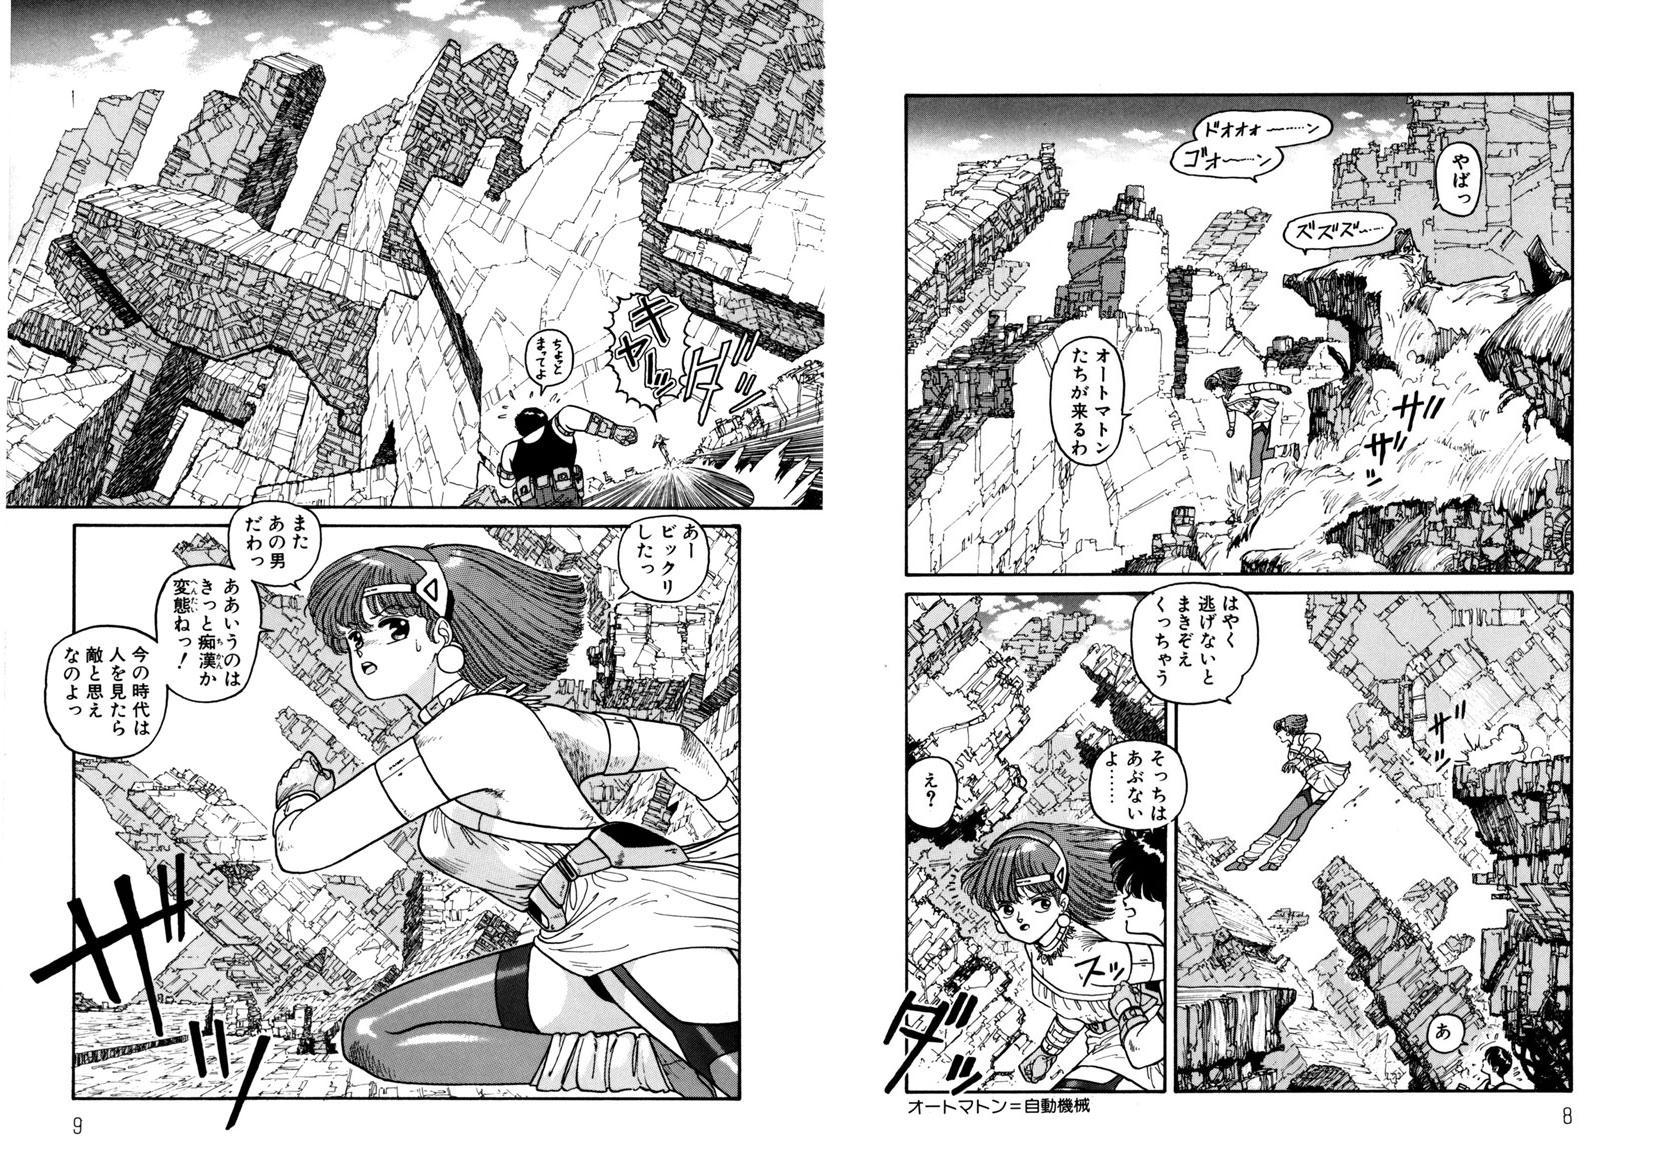
\includegraphics[width=0.9\linewidth]{pict/02/ARMS003.jpg}
   \caption{Manga109Dataset に含まれる漫画画像の例（『ARMS』より）．© 加藤 雅基／東京三世社}
   \label{fig:manga109example}
\end{figure}

% ▼▼▼ 仕掛け：main じゃないとき（単体のとき）だけ参考文献を表示 ▼▼▼
\ifdefined\ismain\else
   \printbibliography[title=参考文献]
\fi
% ▲▲▲▲▲▲▲▲▲▲▲▲▲▲▲▲▲▲▲▲▲▲▲▲▲▲▲▲▲▲▲▲▲▲▲▲

\end{document}